\chapter{Interfejs graficzny - strona internetowa}
Widok serwisu dla nie zalogowanego użytkowika można zobaczyć na rysunku \ref*{fig:strona_glowna} na stronie \pageref{fig:strona_glowna}
\begin{figure}[H]
	\centering
	\includegraphics[width=17cm, height=10cm] {fig/interfejs}
	\caption{Interfejs - strona główna}
	\label{fig:strona_glowna}
\end{figure}
Kod pliku wejściowego strony \s!index.php!, na który przekierowywane są wszystkie zapytania z serwisu poprzez moduł \s!mod_rewrite! (ustawienia w pliku \s!.htaccess!) możemy zobaczyć poniżej\\
\begin{lstlisting}[language=PHP]
<?php 
session_start();
include('class/database.php');
$DB = database::instance();
include('class/upr.php');
include('ctrl/functions.php');
include('class/klient.php');
include('class/koszyk.php');
include('class/transakcja.php');
sprawdz_uprawnienia();

if(!isset($_GET['site'])) $_GET['site']='';
include('ctrl/drzewo-kategorii.php');
ob_start();
switch($_GET['site']) {
case 'logout': 
	session_destroy();
	header("Location: {$dir}glowna.html");
	break;
case 'index':
case '':
	header("Location: {$dir}glowna.html");
	break;
case 'glowna':
	include('view/glowna.php'); 
	break;
case 'produkt':
	include('ctrl/produkt.php');
	$htitle = 'Lista produktów';
	include('view/produkt.php');
	break;
case 'koszyk':
	include('ctrl/koszyk.php');
	$htitle = 'Twój koszyk';
	include('view/koszyk.php');
	break;
case 'login':
	if(isset($_POST['login']) AND isset($_POST['password'])) 
		include('ctrl/login.php');
	$htitle = 'Klient - logowanie';
	include('view/logowanie.php'); 
	break;
case 'login-pracownik':
	...
case 'kategoria':
	...
case 'produkt-edycja':
	...
case 'produkt-edycja-lista':
	...
case 'rejestracja':
	...
case 'profil':
	...
case 'baza_klientow':
	...
case 'transakcja': 
	...
default:
	header("Location: {$dir}glowna.html");
	exit;
}
$content = ob_get_contents();
ob_end_clean(); 
include('view/view.php'); 
/**/
?>
\end{lstlisting}

Wykorzystywane klasy:
\begin{itemize}
\item Baza danych w modelu singletona (model, gdzie może istnieć tylko jedna instancja obiektu danej klasy)
\begin{lstlisting}[language=PHP]
class database extends mysqli{
static $THIS; //instancja singletona

private $host 	= 'localhost';
private $login 	= 'interfejs';
private $pass 	= '******';
private $db 	= 'projekt_bazy_sklep';

private function __construct(){
	parent::__construct($this->host, $this->login, 
		$this->pass, $this->db);
}

static function instance(){
	if(empty(self::$THIS) OR !self::$THIS->ping()) {
		self::$THIS = new database();
		self::$THIS->query('SET NAMES \'utf8\'');
	}
	return self::$THIS;
}
}
\end{lstlisting}
	\item Klasa klient
\begin{lstlisting}[language=PHP]
class klient {
	static $zalogowany;
	static $login;
	static $klient_id;
	static $typ;
	static $imie;
	static $nazwisko;
	static $NIP;
	static $nazwa_firmy;
	static $dom_adr_wys;
	
	static function wyciagnij_dane() {
	...
\end{lstlisting}
\item Koszyk
\begin{lstlisting}[language=PHP]
class koszyk {
	static function &produkty() { ... }
	static function dodaj($produkt_id, $sztuk) { ... }
	static function usun($produkt_id) { ... }
}
\end{lstlisting}
\item Uprawnienia
\begin{lstlisting}[language=PHP,showstringspaces=false]
class upr {
	const pracownik	= 'pracownik';
	const kategoria = 'kategoria';
	const produkt	= 'produkt';
	const wysylka = 'wysylka';
	const klient = 'klient';
	const raport = 'raport';
	
	static function maUprawnienia($upr) {
		...
	}
	
	static function wyrzucBezUprawnien($upr) {
		if(self::maUprawnienia($upr)) return;
		putMessage('Nie masz uprawnień 
			do przeglądania tej zawartości');
		header("Location: {$dir}glowna.html");
		exit;
	}
	static function wyrzucStad() {
		putMessage('Nie masz uprawnień do 
			przeglądania tej zawartości');
		header("Location: {$dir}glowna.html");
		exit;
	}
}
\end{lstlisting}
\end{itemize}

Każdą z podstron obsługują dołączane z poziomu \s!index.php!:
\begin{itemize}
	\item Kontroler - plik z folderu \s!ctrl!, zawierający zapytania do bazy danych i warunkowe wykonanie instrukcji takich jak modyfikacja czy wprowadzanie danych. Przykładowy fragment takiego pliku:
\begin{lstlisting}[language=PHP]
if(isset($gkat) && is_numeric($gkat)) {
	$DB->real_query("call menu_drzewo_kat($gkat)") 
		OR die($DB->error);
	$resultSets = array();
	$i = 0;
	do {
		if ($res = $DB->store_result()) {
			$resultSets[$i++] = 
				$res->fetch_all(MYSQLI_ASSOC);
			$res->free();
		} else if($DB->errno)
		putMessage($DB->error);
	} while ($DB->more_results() && $DB->next_result());
	for($l=count($resultSets)-1; $l>=0; $l--) {
		foreach($resultSets[$l] as $row) putKat($row);
	}
}
\end{lstlisting}
	\item Widok - plik z folderu \s!view! zawierający głównie elementy \s!HTML!, tj częsci definiującej wygląd, przykład zawartości:
\begin{lstlisting}[language=HTML,showstringspaces=false]
<h2>Klient - logowanie</h2>
<p>Aby zalogować się na konto, wprowadź login i hasło</p>
<form class="formularz" action="login.html" method="post" >
<ul>
	<li>
	<label for="login">Login</label>
	<input type="text" name="login" value="<?php
	 if(isset($_POST['login']))echo $_POST['login']; ?>" >
	</li>
	<li>
	<label for="password">Hasło</label>
	<input type="password" name="password" value="<?php
	 if(isset($_POST['password'])) echo $_POST['password']; ?>" >
	</li>
	<li>
	<input type="submit">
	</li>
</ul>
</form>
\end{lstlisting}
\end{itemize}
Menu serwisu dla niezalogowanego użytkownika przedstawia rysunek \ref{fig:nie_zalogowany} na stronie \pageref{fig:nie_zalogowany}. Dostepne jest 
\begin{itemize}
	\item Przejście do strony głównej
	\item Przeglądanie kategorii oraz produktów 
	\item Rejestracja
	\item Logowanie
\end{itemize}


\begin{figure}[H]
	\centering
	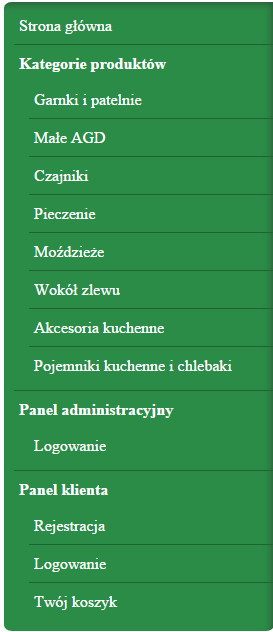
\includegraphics {fig/menu_nie_zalogowany}
	\caption{Widok menu dla niezalogowanego użytkownika}
	\label{fig:nie_zalogowany}
\end{figure}
Po kliknięciu na kategorii która zawiera podkategorie następuje rozwinięcie menu. Efekt widoczny na screenie \ref{fig:menu_rozwijalne} na stronie \pageref{fig:menu_rozwijalne}
\begin{figure}[H]
	\centering
	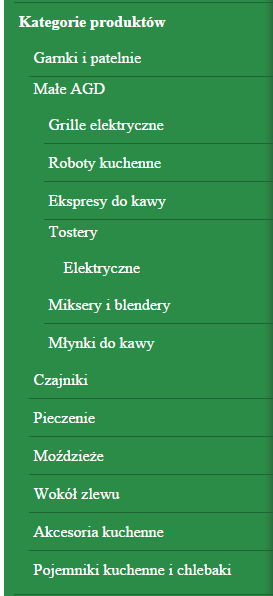
\includegraphics {fig/menu_rozwijanie}
	\caption{Rozwijanie menu}
	\label{fig:menu_rozwijalne}
\end{figure}

Formularz logowania pracownika widoczny na \ref{fig:pracownik_logowanie} na stronie \pageref{fig:pracownik_logowanie}
\begin{figure}[H]
	\centering
	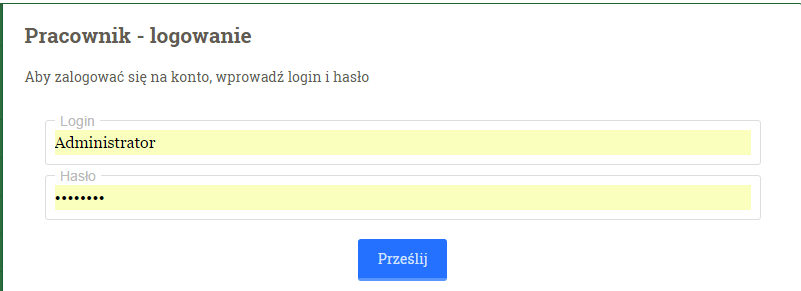
\includegraphics[width=15 cm] {fig/pracownik_logowanie}
	\caption{Formularz logowania dla pracownika}
	\label{fig:pracownik_logowanie}
\end{figure}
Po zalogowaniu na konto pracownika w \textit{Panelu administracyjnym}
pojawiają sie nowe opcje widoczne  na rysunku \ref{fig:panel_pracownik} na stronie \pageref{fig:panel_pracownik} 
\begin{figure}[H]
	\centering
	\includegraphics {fig/pracownik_logowanie_panel}
	\caption{Opcje dostępne po zalogowaniu na konto pracownika}
	\label{fig:panel_pracownik}
\end{figure}
Opcja \textit{Dodaj/edytuj kategorie} pozwala na dodawanie kategorii rys.\ref{fig:dod_kat} strona \pageref{fig:dod_kat} lub edycje rys\ref{fig:e_kat} strona \pageref{fig:e_kat}
\begin{figure}[H]
	\centering
	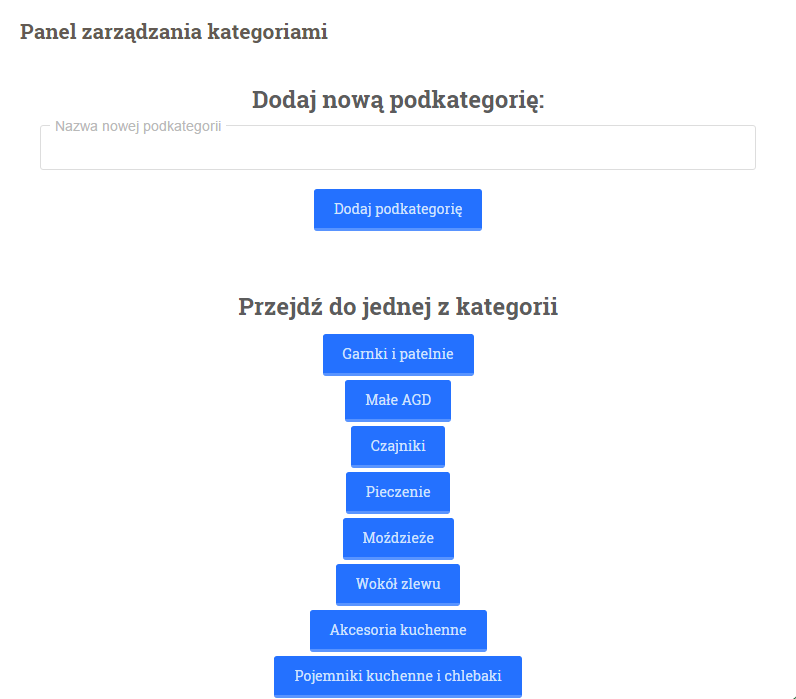
\includegraphics [width=15cm] {fig/dodawanie_kat}
	\caption{Formularz dodawania kategorii}
	\label{fig:dod_kat}
\end{figure}
\begin{figure}[H]
	\centering
	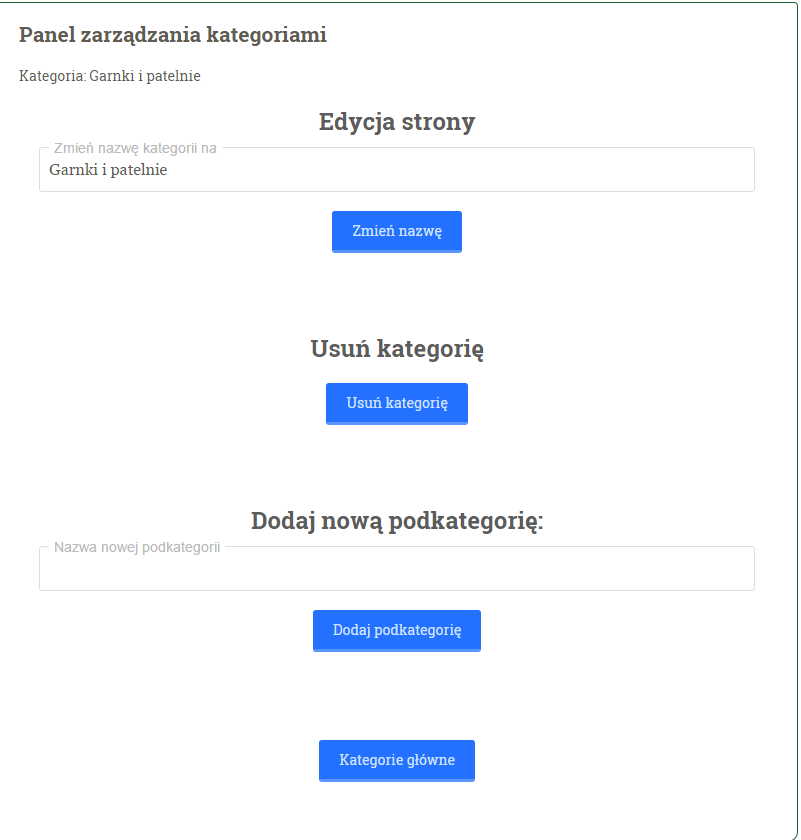
\includegraphics [width=15cm]{fig/edycja_kategorii}
	\caption{Panel edycji kategorii}
	\label{fig:e_kat}
\end{figure}
 Panel zarządzania produktami rys.\ref{fig:dod_prod}pozwala na
 \begin{enumerate}
 	\item Dodanie nazwy produktu
 	\item Dodanie opisu za pomocą zaimpementowanego w projekcie edytora
 	\item Wybór kategorii z listy istniejących kategorii
 	\item Ustalenie ceny produktu
 	\item Określemie ilości sztuk dodawanych do magazynu
 	
 \end{enumerate}
 
\begin{figure}[H]
	\centering
	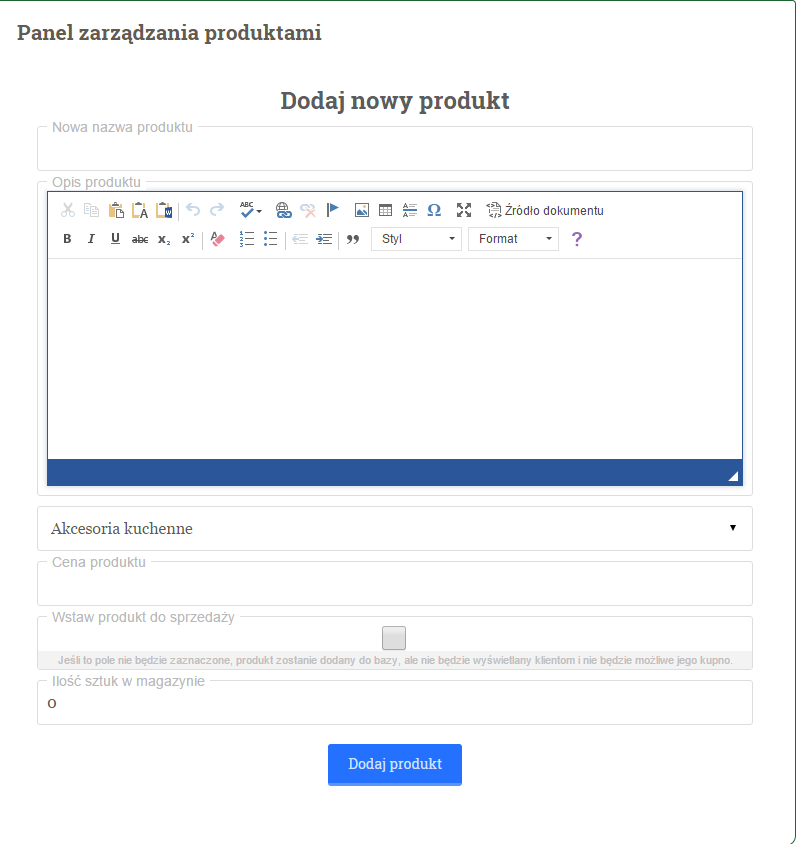
\includegraphics [width=15cm] {fig/dodawanie_produktu}
	\caption{Formularz dodawania produktu}
	\label{fig:dod_prod}
\end{figure}
Zakladka \textit{Baza klientów} wyswietla listę kont zarejestrowanych klientów z podziałem na \begin{enumerate}
	\item Klientów indywidualnych
	\item Konta firmowe
\end{enumerate}
Wyświetlane są podstawowe dane, dla klientów indywidualnych: imie, nazwisko. Dla kont firmowych: nazwa firmy i NIP. Jeżeli użytkownik nie uzupełnił danych na swój temat wyświetlony zostanie odpowiednia informacja w nawiasach \{ \}.
\begin{figure}[H]
	\centering
	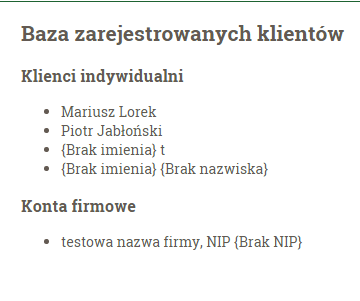
\includegraphics {fig/baza_klientow}
	\caption{Baza klientów}
	\label{fig:baza_klient}
\end{figure}
Formularz rejstracyjny dla klientów, wymaga:
\begin{itemize}
\item Wybranie typu konta: \textit{Osoba prywatna} lub \textit{Firma}
\item login - wymagane jest aby był unikalny
\item hasło	
\end{itemize}
\begin{figure}[H]
	\centering
	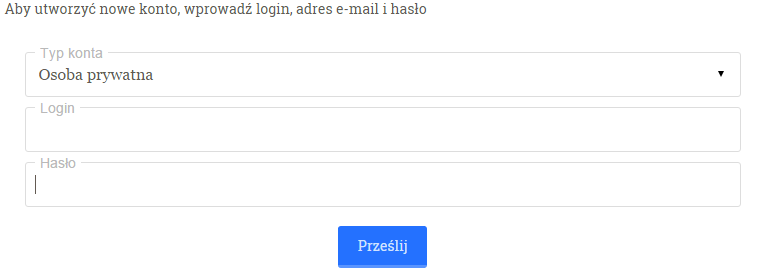
\includegraphics [width=15cm] {fig/rejestracja}
	\caption{Formularz rejestracji}
	\label{fig:rejestracja}
\end{figure}
Po zalogowaniu pojawi w \textit{Panelu Klienta} pojawia się opcja \textit{Ustawienia konta}
widoczne na rys.\ref*{fig:profil_zarz} na stronie \pageref{fig:profil_zarz} Możliwa jest edycja podstawowych danych oraz zmiana hasła do konta
\begin{figure}[H]
	\centering
	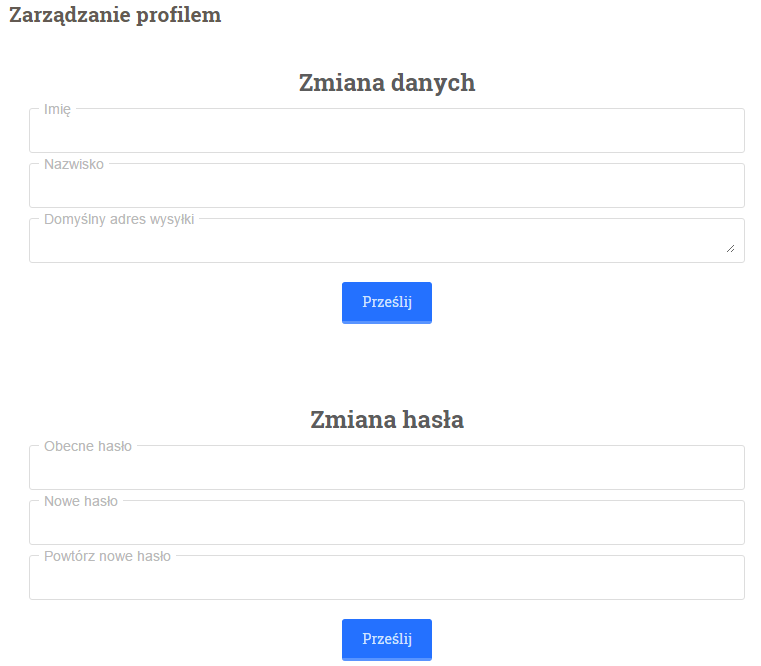
\includegraphics [width=15cm]{fig/zarzadzanie_profilem}
	\caption{Formularz zarzadzania profilem użytkownika}
	\label{fig:profil_zarz}
\end{figure}